\FloatBarrier
\subsection{Question 4}
Direct adaptive controller codebase is presented in \autoref{code:sstr41}. As shown in \autoref{fig:sstr41}, the system is stable and in \autoref{fig:sstr42}, cummulative loss of the system is bounded. \autoref{fig:sstr43} presents the parameters estimation plot of direct adaptive controller.

\begin{code}
	\begin{matlabcode}{firstnumber = 1}
run('SSTR_0.m');

%%  Solve Diophantine equation
[F,G] = diophantine(A,C,1);

%%  Closed loop system
G_ol = minreal(G_discrete*tf(A,conv(B,F),Ts));

%%  closed loop system
G_cl = feedback(G_ol,1);
[B_true,A_true] = tfdata(G_cl,'v');

%% Simulation settings
na = length(A_true)-1; nb = length(B_true)-1;
N = 31;              
theta = zeros(nb + na, 1);  
gamma = 0.01;          

u = ones(1,N);
y = zeros(1,N);
y_ref = ones(1,N);
phi = zeros(nb + na, 1);

%% Simulation loop
for k = 4:N
e = y_ref(k) - y(k);  
phi = [-y(k-1); -y(k-2); -y(k-3); u(k-1); u(k-2); u(k-3)];
u(k) = theta' * phi;
y(k) = -A_true(2)*y(k-1) - A_true(3)*y(k-2) - A_true(4)*y(k-3) + ...
B_true(2)*u(k-1) + B_true(3)*u(k-2) + B_true(4)*u(k-3);

theta = theta - gamma * e * phi;
THETA(:,k) = theta; 
end
	\end{matlabcode}
	\captionof{listing}{Direct adaptive implementation of minimum variance controller}
	\label{code:sstr41}
\end{code}

\begin{figure}
	\centering
	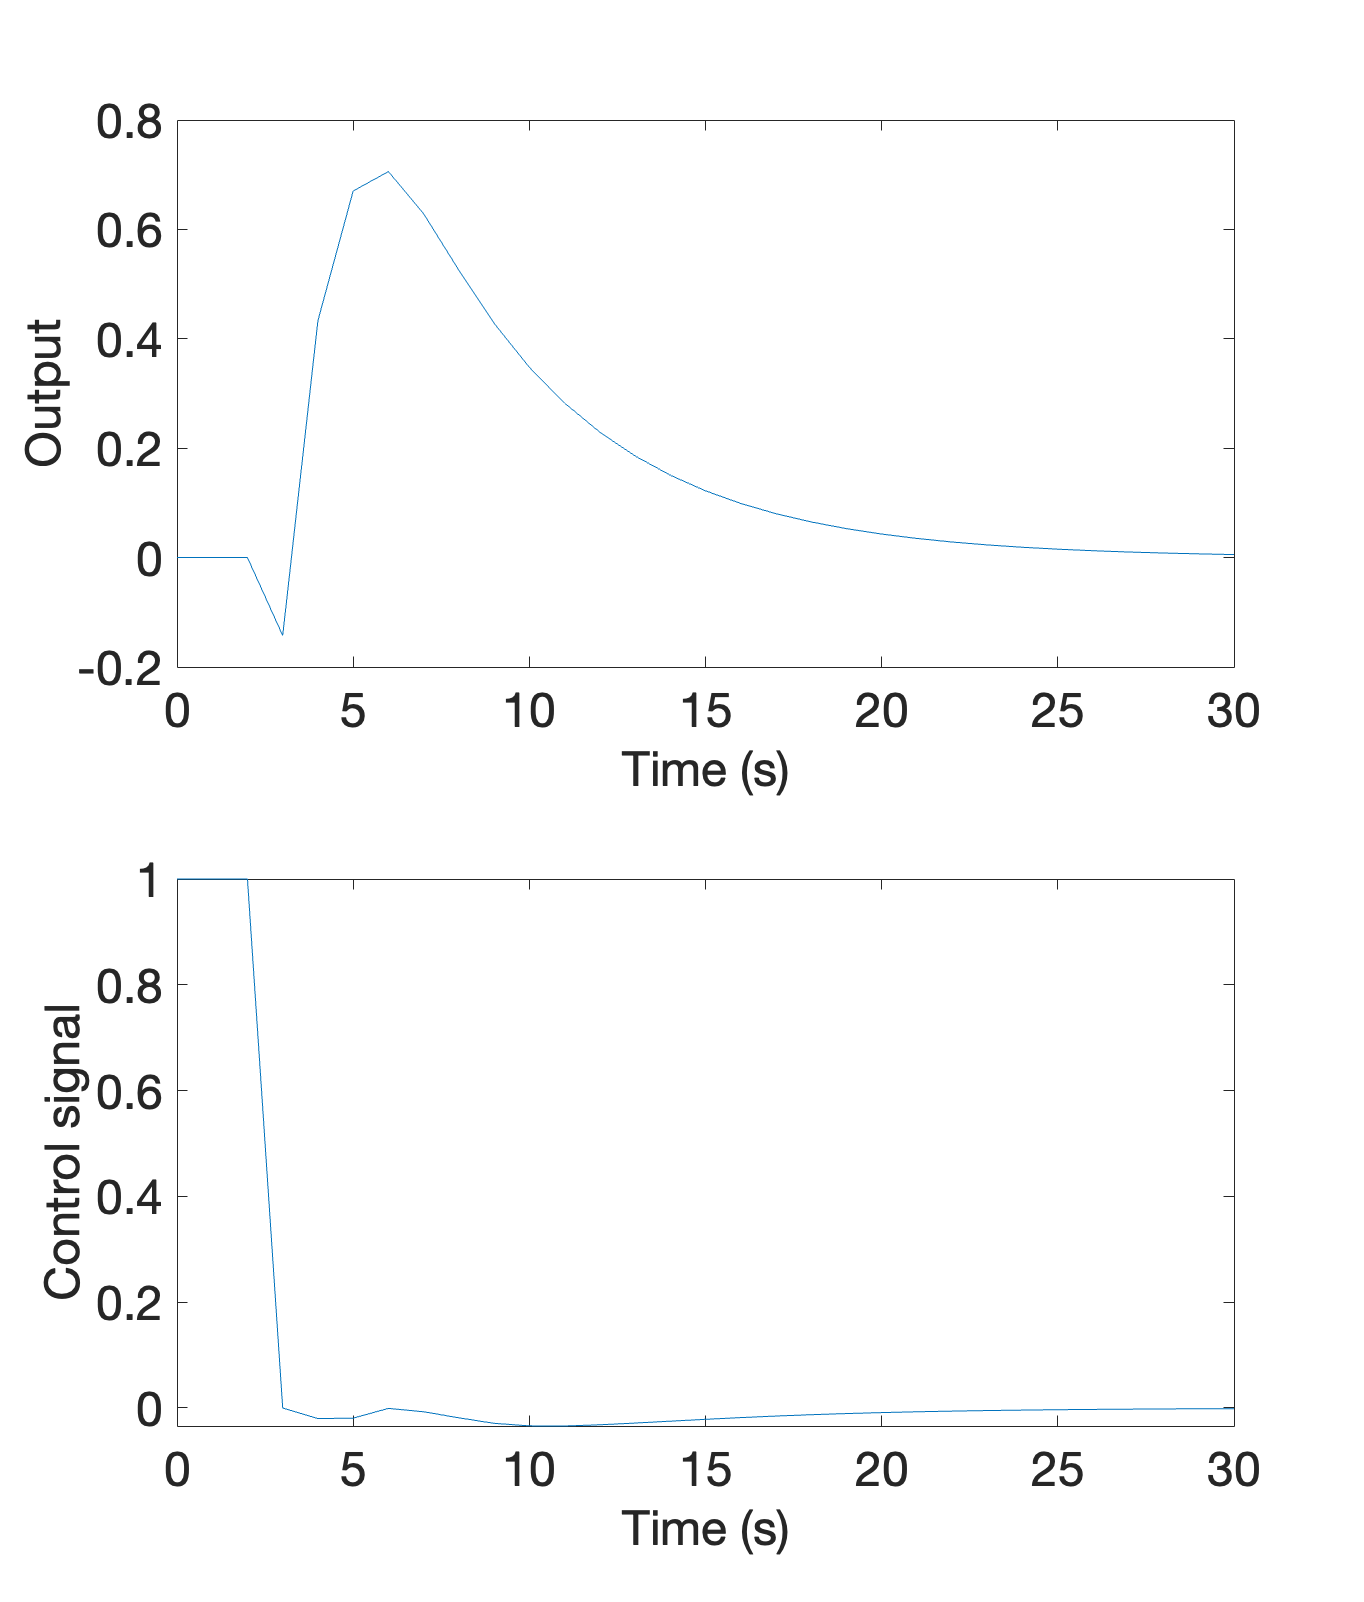
\includegraphics[width=\textwidth]{images/sstr41.png}
	\caption{output and control of direct adaptive implementation of minimum variance controller}
	\label{fig:sstr41}
\end{figure}

\begin{figure}
	\centering
	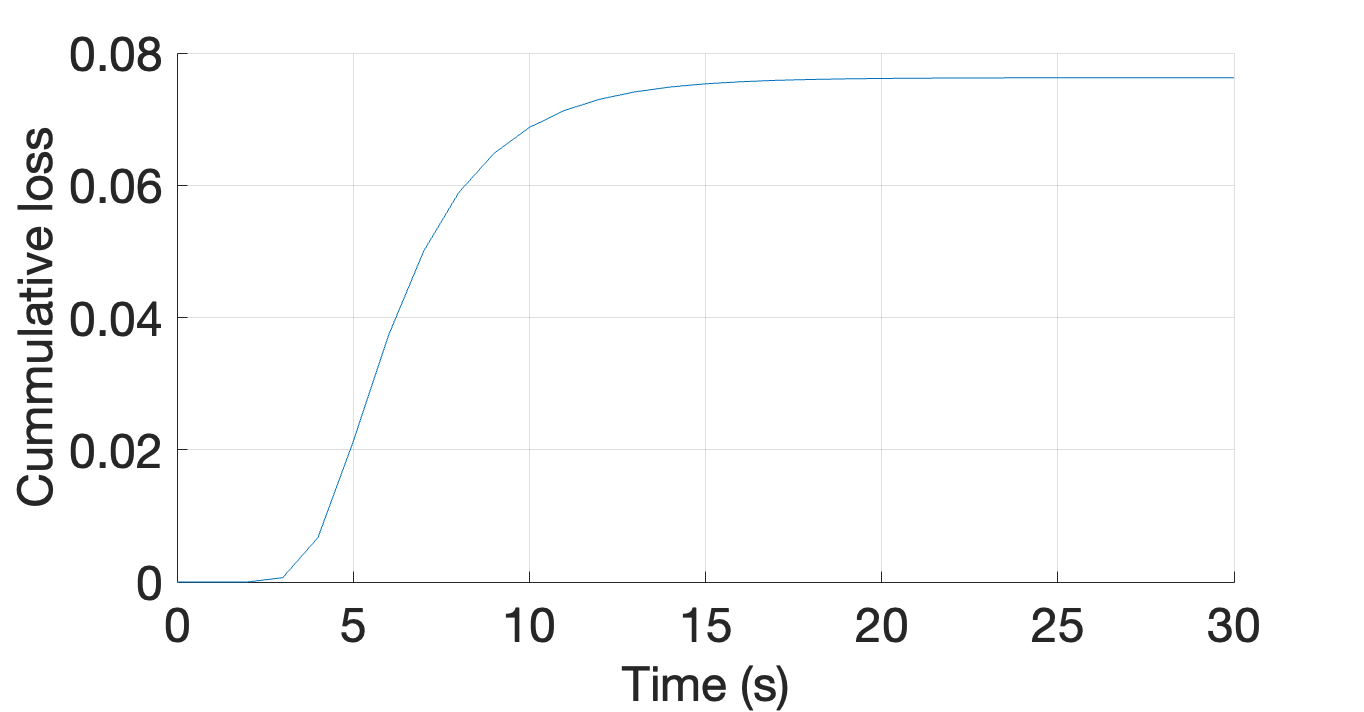
\includegraphics[width=\textwidth]{images/sstr42.png}
	\caption{Cummulative loss of direct adaptive implementation of minimum variance controller}
	\label{fig:sstr42}
\end{figure}

\begin{figure}
	\centering
	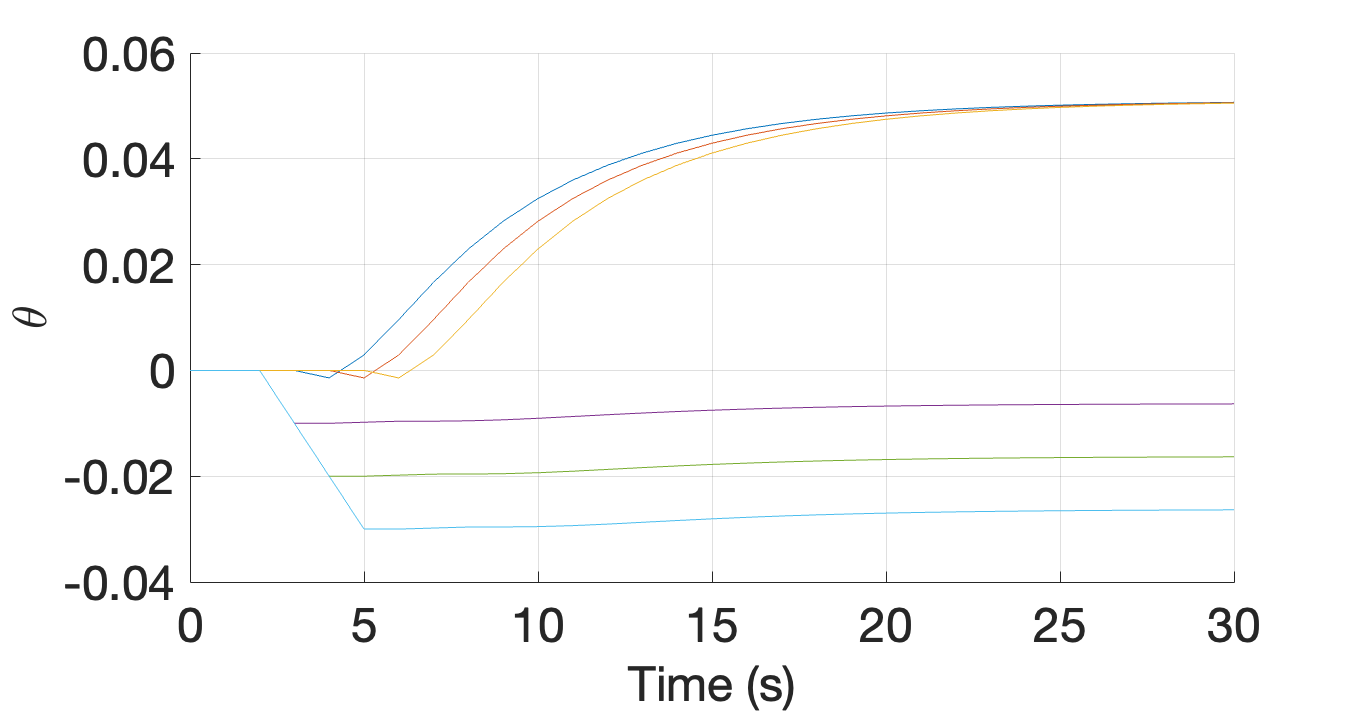
\includegraphics[width=\textwidth]{images/sstr43.png}
	\caption{Estimated parameters of direct adaptive implementation of minimum variance controller}
	\label{fig:sstr43}
\end{figure}

\noindent The code for this section is available at \lstinline|assignment3/SSTR/SSTR_4.m|. 
